\chapter{Reti neurali (parte 2): addestramento in pratica}\label{ch-08}

Con la backpropagation
(\href{07\%20-\%20Note\%20sulla\%20backpropagation}{07 - Note sulla
backpropagation}) sappiamo calcolare il gradiente per ogni peso della
rete. Questa lezione affronta tutte le questioni pratiche che servono
per addestrare davvero un MLP: inizializzazione, minimi multipli,
versioni on-line/batch/mini-batch, learning rate e momentum, criteri di
arresto, overfitting e regolarizzazione, numero di unità (con il Cascade
Correlation), rappresentazione di input e output. Chiude una sintesi di
pregi e difetti delle reti neurali e i primi consigli per il progetto
(benchmark MONK).

\begin{figure}[htbp]
\centering
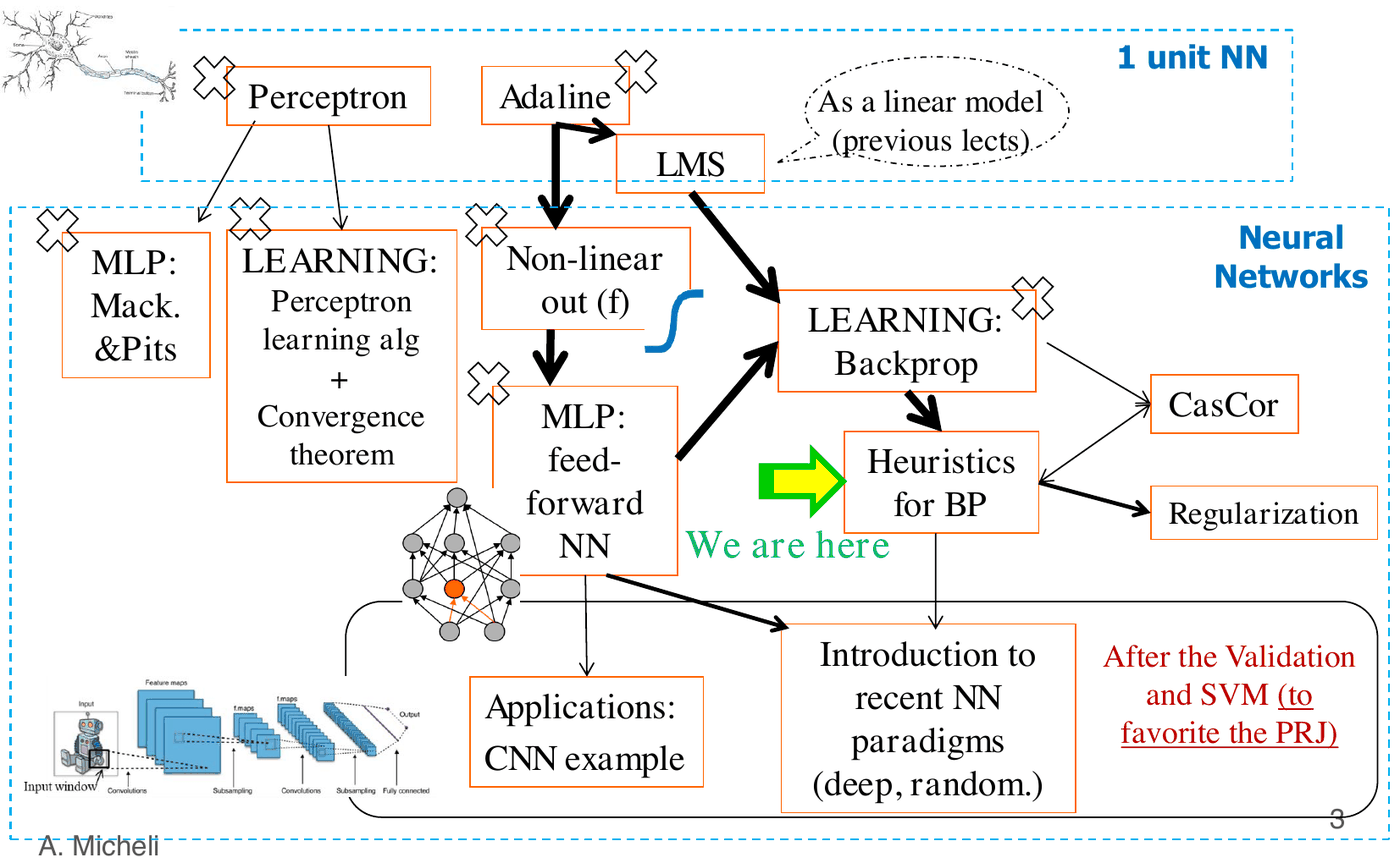
\includegraphics[width=0.91\linewidth,height=0.42\textheight,keepaspectratio]{images/08-nn2_mappa.png}
\caption{Zoom sul blocco ``reti neurali'' del corso.}
\end{figure}

\section{Filosofia}\label{filosofia}

Il ML si è evoluto da una collezione di trucchi euristici a quadri
concettuali generali: il professore preferisce non introdurre troppi
dettagli euristici. Molte delle tecniche che seguono si possono
esplorare sperimentalmente nel progetto; alcune hanno un fondamento
teorico (la regolarizzazione) e si applicano in un quadro più generale.
Quelle indicate con \textbf{(!)} sono molto comuni e \textbf{vanno
usate} nel progetto.

\begin{boxwarning}{Diffidare delle ``regole empiriche''}

Evitare le \emph{rules of thumb} trovate sui blog, a meno che non siano
dimostrate in articoli scientifici o non se ne sia verificato
sperimentalmente il vantaggio.

\end{boxwarning}

\begin{boxtip}{Un'interpretazione utile}

La backpropagation è un \textbf{percorso nello spazio dei pesi} (sulla
superficie della loss). Il percorso dipende da: i dati, il modello, il
\textbf{punto di partenza} (pesi iniziali), la \textbf{velocità di
convergenza} e il \textbf{punto finale} (regola di arresto). Tutte
queste scelte costituiscono un \textbf{controllo della ricerca} nello
spazio delle ipotesi.

\end{boxtip}

L'algoritmo di base resta la discesa del gradiente: pesi iniziali
piccoli, \(\Delta\mathbf{w} = -\partial E/\partial\mathbf{w}\)
(calcolato con la backprop: fase forward fino alle uscite, poi fase
backward per i delta),
\(\mathbf{w}_{new} = \mathbf{w} + \eta\,\Delta\mathbf{w}\), ripetere. Il
modello è spesso \textbf{sovra-parametrizzato} e l'ottimizzazione è
\textbf{non convessa} e potenzialmente instabile: da qui le questioni
che seguono. Gli \textbf{iperparametri} sono i valori che bisogna
fissare per eseguire l'addestramento.

\section{Valori iniziali dei pesi}\label{valori-iniziali-dei-pesi}

\begin{boxtip}{(!) Inizializzazione}

Inizializzare i pesi con \textbf{valori casuali vicini a zero}, ad
esempio nell'intervallo \([-0{,}7;\ +0{,}7]\) (per dati standardizzati).

\end{boxtip}

Da evitare:

\begin{itemize}
\tightlist
\item
  \textbf{tutti zero}: i delta delle unità nascoste sarebbero tutti
  nulli (dipendono dai pesi verso l'uscita) e la rete non imparerebbe;
\item
  \textbf{valori alti}: le sigmoidi partono \textbf{saturate}, con
  derivate quasi nulle e apprendimento lentissimo;
\item
  \textbf{tutti uguali}: le unità nascoste restano \textbf{simmetriche}
  (ricevono gli stessi aggiornamenti e calcolano tutte la stessa cosa).
  La casualità serve a \textbf{rompere la simmetria}.
\end{itemize}

Si può tenere conto del \textbf{fan-in} (numero di input di un'unità),
ad esempio con un intervallo pari a
\(\text{range}\cdot 2/\text{fan-in}\), ma non se il fan-in è troppo
grande e non per le unità di uscita (altrimenti i delta partono vicini a
zero). Molto popolare è l'inizializzazione di \textbf{Glorot e Bengio}
(2010): bias a 0 e pesi da una distribuzione uniforme in
\([-1/a, +1/a]\) con \(a = \sqrt{\text{fan-in}}\) (o, in risultati
successivi, \(a\) dipendente anche dal fan-out).

\begin{boxnote}{(!) Per il progetto}

Una rete molto piccola (pochissime unità) può dipendere fortemente
dall'inizializzazione.

\end{boxnote}

\section{Minimi multipli}\label{minimi-multipli}

La loss \textbf{non è convessa}: ci sono molti minimi locali, e il
risultato dipende dai pesi iniziali. Quindi:

\begin{boxtip}{(!) Più inizializzazioni}

Provare diverse configurazioni iniziali casuali (ad esempio 5--10 o più
\emph{trial}). Per valutare il modello si riporta la \textbf{media} dei
risultati (media degli errori) e la \textbf{varianza}. Se si vuole
un'unica risposta, si può scegliere la soluzione con il più basso errore
di validazione (o la mediana), oppure sfruttare i diversi punti finali
con una risposta \textbf{di comitato} (media delle uscite o voto). Più
avanti si vedrà perché gli \emph{ensemble} sono vantaggiosi in generale.

\end{boxtip}

Fermarsi in un minimo locale con errore troppo alto non è un grosso
problema: si vede l'errore finale e si può ricominciare. Spesso un
\textbf{``buon'' minimo locale è sufficiente}.

\subsection{Serve davvero il minimo
globale?}\label{serve-davvero-il-minimo-globale}

Due osservazioni fondamentali:

\begin{enumerate}
\def\labelenumi{\arabic{enumi}.}
\tightlist
\item
  Nel ML \textbf{non cerchiamo né il minimo locale né quello globale di
  \(R_{emp}\)}, ma il minimo di \(R\), che non possiamo calcolare.
  Spesso ci si ferma in un punto che non ha nemmeno gradiente nullo.
\item
  La rete è uno \textbf{spazio delle ipotesi di dimensione variabile}:
  durante l'addestramento la VC-dim cresce, l'errore di training scende
  verso zero (o il minimo globale) mentre la rete diventa troppo
  complessa. Bisogna fermarsi \textbf{prima} di questa condizione di
  \emph{overtraining} (e quindi overfitting), indipendentemente dalla
  questione minimi locali/globali.
\end{enumerate}

\section{On-line, batch e mini-batch}\label{on-line-batch-e-mini-batch}

Ricordiamo (vedi i modelli lineari):

\begin{itemize}
\tightlist
\item
  \textbf{Batch}: si sommano i gradienti di tutti i pattern di
  un'\textbf{epoca} (un ciclo completo di presentazione del training
  set) e poi si aggiornano i pesi.
\item
  \textbf{On-line/stocastico}: si aggiorna \(\mathbf{w}\) dopo ogni
  pattern \(p\) con \(\Delta_p\mathbf{w}\), senza aspettare la somma.
  Progredisce a ogni esempio, può essere più veloce, ma richiede
  \(\eta\) più piccolo.
\end{itemize}

In formule, per il peso \(w_{tu}\): \[
\text{batch: } -\frac{\partial E}{\partial w_{tu}} = -\sum_{p=1}^{l}\frac{\partial E_p}{\partial w_{tu}} = \sum_{p=1}^{l}\delta_{p,t}\,o_{p,u}, \qquad \text{on-line: } -\frac{\partial E_p}{\partial w_{tu}} = \delta_{p,t}\,o_{p,u}.
\]

\begin{boxabstract}{Batch e on-line a confronto}

\textbf{Batch} --- 1) fissare \(\mathbf{w}_{init}\) ed \(\eta\); 2)
calcolare \(\Delta\mathbf{w}\) sull'intero training set (la somma su
\(p\) è dentro questo passo); 3)
\(\mathbf{w}_{new} = \mathbf{w} + \eta\,\Delta\mathbf{w}\); 4) ripetere
fino a convergenza.

\textbf{On-line} --- 1) fissare \(\mathbf{w}_{init}\) ed \(\eta\); per
ogni pattern \(p\): 2) calcolare \(\Delta_p\mathbf{w}\); 3)
\(\mathbf{w}_{new} = \mathbf{w} + \eta\,\Delta_p\mathbf{w}\); 4)
ripetere (epoca dopo epoca) fino a convergenza.

\end{boxabstract}

Il batch dà una stima \textbf{più accurata} del gradiente. Nell'on-line
il gradiente di un singolo pattern è un'approssimazione
\textbf{rumorosa} del gradiente complessivo, da cui il nome
\emph{stochastic gradient descent}: la discesa procede a zig-zag, il che
\textbf{può aiutare a sfuggire ai minimi locali}.

\begin{boxtip}{(!) Shuffling}

Nella versione on-line bisogna presentare i pattern in \textbf{ordine
diverso} a ogni epoca (di solito \textbf{mescolandoli casualmente}), per
evitare una deriva sistematica nella discesa.

\end{boxtip}

\begin{figure}[htbp]
\centering
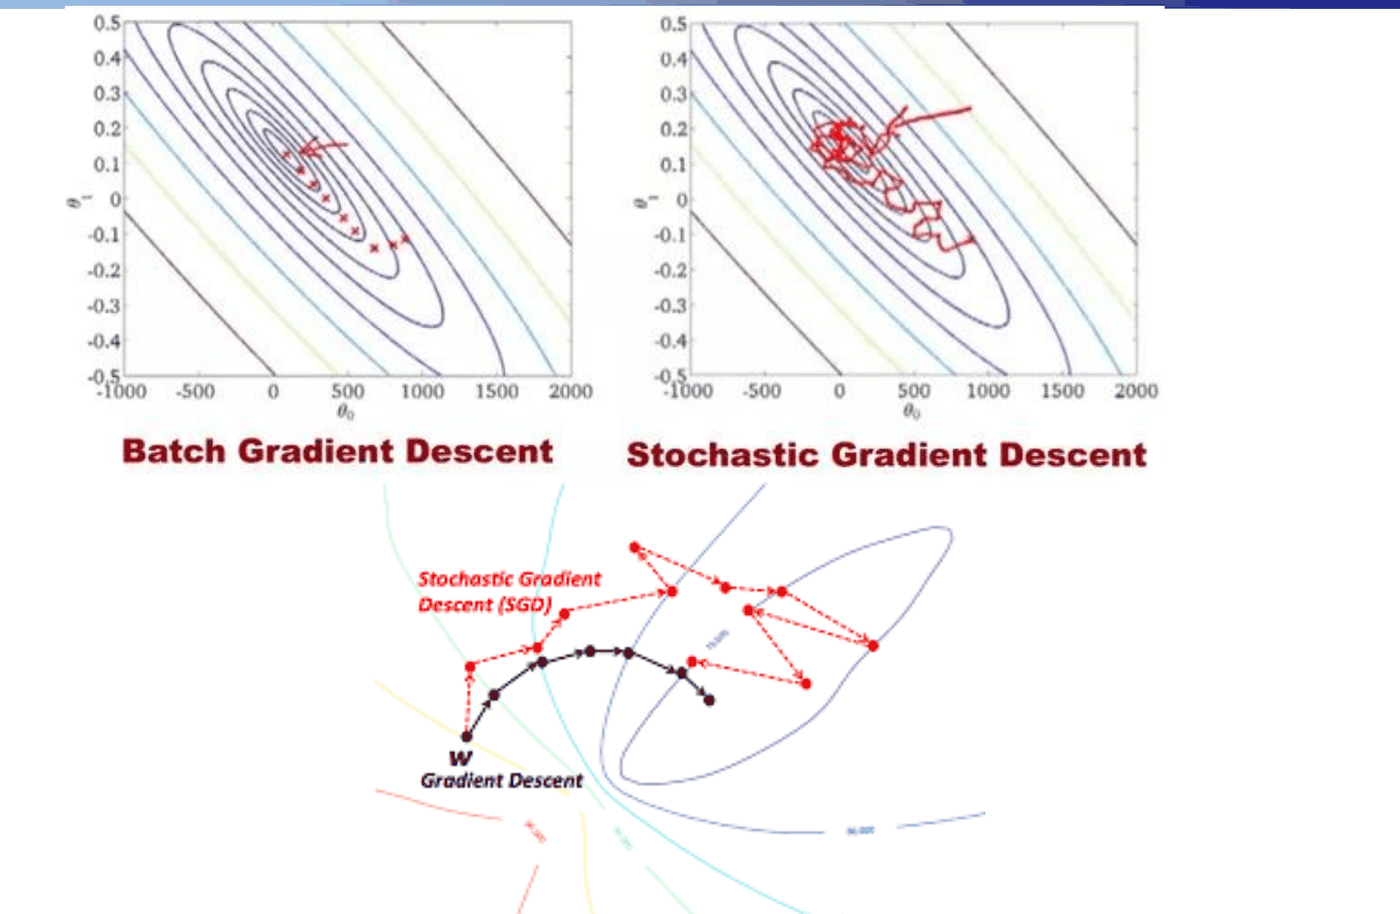
\includegraphics[width=0.71\linewidth,height=0.42\textheight,keepaspectratio]{images/08-nn2_sgd-vs-batch.png}
\caption{Discesa del gradiente batch e stocastica.}
\end{figure}

\subsection{Mini-batch}\label{mini-batch}

Nel \textbf{mini-batch} si divide ogni epoca in parti: si sommano i
gradienti di \(mb\) pattern (\(1 < mb < l\)) prima di aggiornare i pesi,
e si ripete finché tutti i dati dell'epoca sono stati usati.
L'aggiornamento avviene quindi a ogni mini-batch invece che a ogni
pattern o a ogni epoca.

\begin{figure}[htbp]
\centering
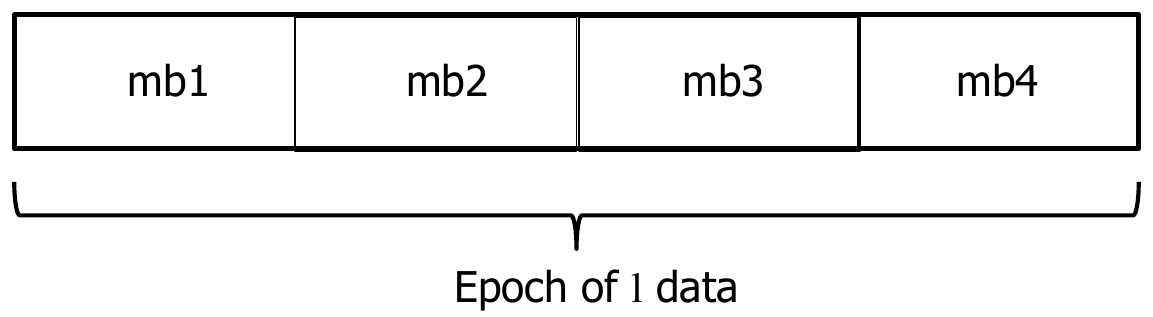
\includegraphics[width=0.60\linewidth,height=0.42\textheight,keepaspectratio]{images/08-nn2_minibatch.png}
\caption{Un'epoca suddivisa in mini-batch.}
\end{figure}

{\def\LTcaptype{none} % do not increment counter
\begin{longtable}[]{@{}
  >{\raggedright\arraybackslash}p{(\linewidth - 4\tabcolsep) * \real{0.3333}}
  >{\raggedright\arraybackslash}p{(\linewidth - 4\tabcolsep) * \real{0.3333}}
  >{\raggedright\arraybackslash}p{(\linewidth - 4\tabcolsep) * \real{0.3333}}@{}}
\toprule\noalign{}
\begin{minipage}[b]{\linewidth}\raggedright
On-line
\end{minipage} & \begin{minipage}[b]{\linewidth}\raggedright
Mini-batch (SGD)
\end{minipage} & \begin{minipage}[b]{\linewidth}\raggedright
Batch
\end{minipage} \\
\midrule\noalign{}
\endhead
\bottomrule\noalign{}
\endlastfoot
non sfrutta il parallelismo tra esempi & compromesso; si adatta alla
memoria della GPU & stima più accurata del gradiente \\
può essere instabile & & più lento (aspetta tutti i dati) \\
il rumore può avere un \textbf{effetto regolarizzante} & & \\
\end{longtable}
}

Il \textbf{mini-batch SGD} usa campionamento casuale (shuffling) per una
stima non distorta del gradiente. Con training set enormi o dati in
streaming si può anche fare a meno delle epoche. Poiché il costo di un
aggiornamento dipende da \(mb\) e non da \(l\), lo SGD con mini-batch è
un fattore chiave per estendere l'apprendimento a dataset di milioni di
esempi.

\section{\texorpdfstring{Il learning rate
\(\eta\)}{Il learning rate \textbackslash eta}}\label{il-learning-rate-eta}

\begin{itemize}
\tightlist
\item
  \textbf{Batch}: gradiente più accurato → si può usare \(\eta\) più
  alto.
\item
  \textbf{On-line}: più veloce ma più instabile → \(\eta\) più piccolo.
\item
  In generale: \(\eta\) \textbf{alto} è veloce ma può essere instabile;
  \(\eta\) \textbf{basso} è stabile ma può essere troppo lento.
  Tipicamente si cerca in \([0{,}01;\ 0{,}5]\) con LMS.
\end{itemize}

\begin{boxtip}{(!) Guardare sempre la curva di apprendimento}

Il grafico dell'errore durante l'addestramento permette di verificare il
comportamento nelle prime fasi di progettazione. Qui si valuta la
\textbf{qualità} della curva e la \textbf{velocità} di convergenza (il
valore assoluto dell'errore dipende anche dalla capacità del modello e
dagli altri iperparametri).

\end{boxtip}

\begin{figure}[htbp]
\centering
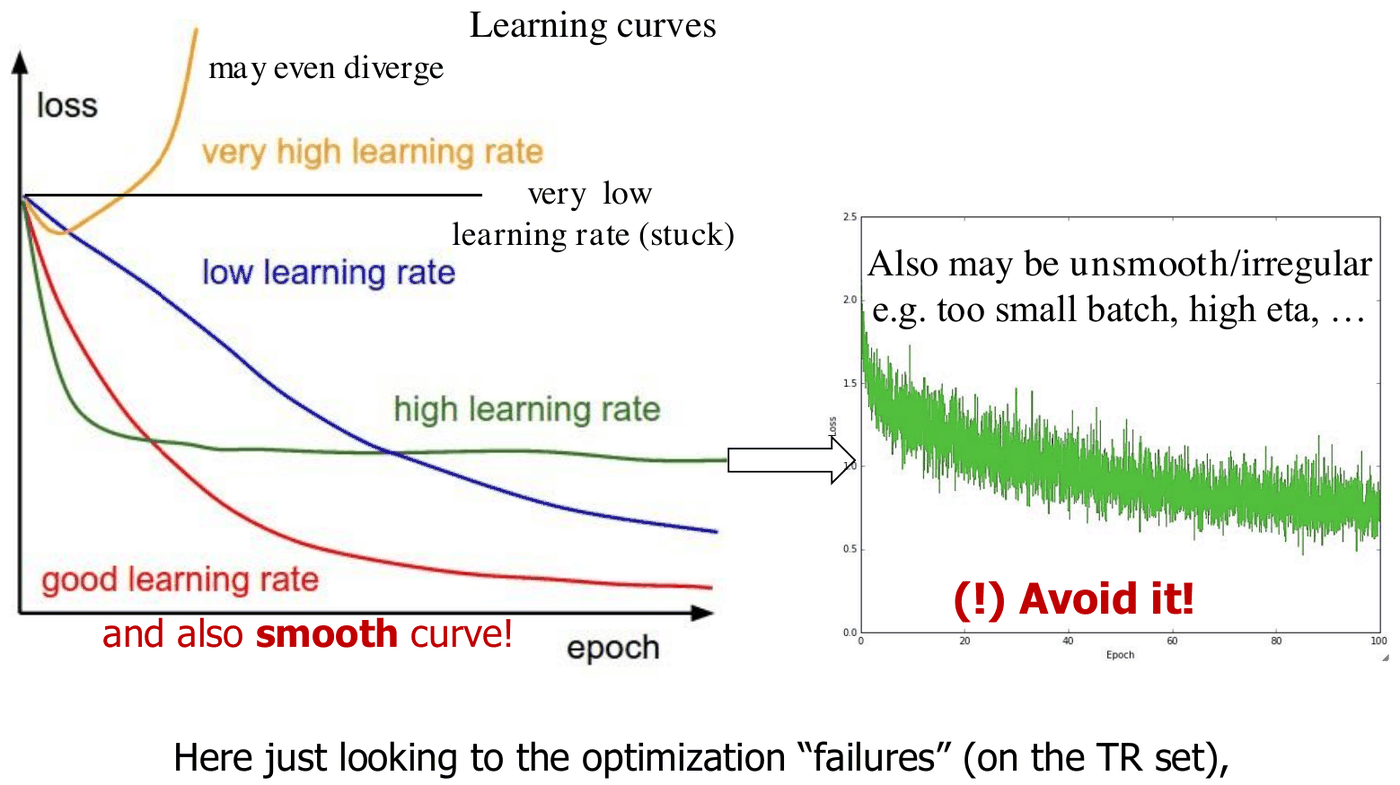
\includegraphics[width=0.91\linewidth,height=0.42\textheight,keepaspectratio]{images/08-nn2_eta.png}
\caption{Effetto del learning rate sulle curve di apprendimento (errore di
training).}
\end{figure}

Una curva irregolare può dipendere da batch troppo piccoli o da \(\eta\)
troppo alto: va evitata. Si cerca una curva che scende rapidamente
\textbf{e in modo liscio}. (Qui si guardano solo i ``fallimenti''
dell'ottimizzazione sul training set, non l'errore di generalizzazione.)

\subsection{\texorpdfstring{LMS: dividere per
\(l\)}{LMS: dividere per l}}\label{lms-dividere-per-l}

\begin{boxtip}{(!) Usare la media dei gradienti}

Conviene usare la \textbf{media} dei gradienti sull'epoca (somma diviso
\(l\)): rende l'approccio uniforme rispetto al numero di dati (è il
\emph{least mean squares}). Equivale a usare \(\eta/l\) con
\(0 < \eta < 1\).

Attenzione: confrontando on-line e batch con LMS, l'on-line richiede un
\(\eta\) \textbf{molto più piccolo} (dello stesso fattore \(1/l\)) per
essere comparabile. Per il mini-batch (se si divide per \(mb\)) va
ritarato \(\eta\), oppure si divide sempre per \(l\).

\end{boxtip}

\subsection{Migliorare la discesa}\label{migliorare-la-discesa}

\subsubsection{Momentum (!)}\label{momentum}

\[
\Delta\mathbf{w}_{new} = -\eta\,\frac{\partial E(\mathbf{w})}{\partial\mathbf{w}} + \alpha\,\Delta\mathbf{w}_{old}, \qquad \mathbf{w}_{new} = \mathbf{w} + \Delta\mathbf{w}_{new},
\] con \(0 < \alpha < 1\) (ad esempio \(0{,}5\)--\(0{,}9\)). Qui
\(\eta\) è incluso in \(\Delta\mathbf{w}\), e dopo ogni passo si salva
\(\Delta\mathbf{w}_{old} = \Delta\mathbf{w}_{new}\).

È il \textbf{metodo della ``palla pesante''} (\emph{heavy ball}): a ogni
passo si aggiunge una frazione dello spostamento precedente, come se i
pesi avessero un'inerzia.

\begin{itemize}
\tightlist
\item
  \textbf{Più veloce nei plateau}: se il gradiente ha lo stesso segno in
  iterazioni consecutive, il momentum aumenta il passo.
\item
  \textbf{Smorza le oscillazioni}: nelle direzioni in cui il gradiente
  cambia segno i contributi si compensano.
\item
  \textbf{Effetto inerzia}: permette di usare \(\eta\) più alti.
\end{itemize}

\begin{figure}[htbp]
\centering
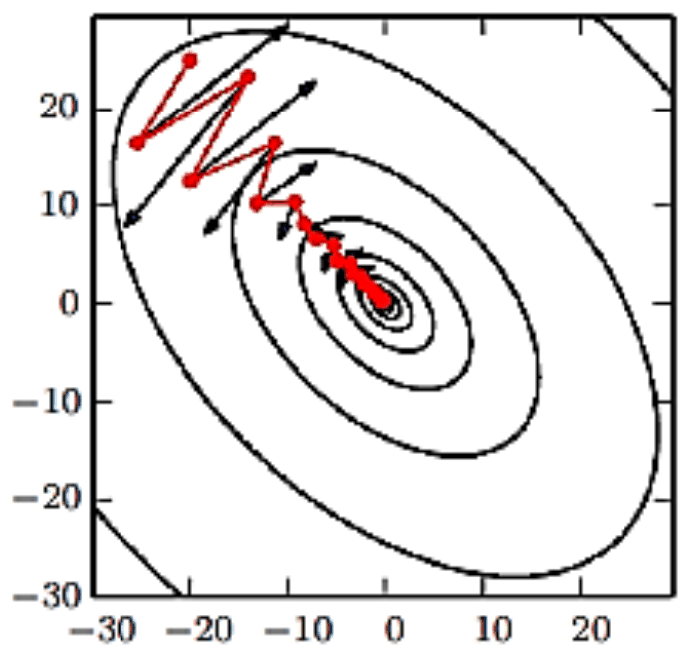
\includegraphics[width=0.46\linewidth,height=0.42\textheight,keepaspectratio]{images/08-nn2_momentum.png}
\caption{Effetto del momentum in un ``canyon'' della superficie d'errore
(Hessiana mal condizionata): il percorso rosso attraversa la valle
invece di rimbalzare tra le pareti.}
\end{figure}

Il momentum nasce per il batch. Nell'on-line \(\Delta\mathbf{w}_{old}\)
è quello del \textbf{pattern precedente}, e il momentum diventa una
\textbf{media mobile dei gradienti passati} che liscia i gradienti
stocastici all'interno dell'epoca (analogamente per il mini-batch). Il
significato è quindi diverso dal batch, dove si combinano gradienti
calcolati sugli stessi esempi in epoche diverse.

\textbf{Nesterov momentum}: si applica prima il momentum
(\(\mathbf{w} + \alpha\Delta\mathbf{w}_{old}\)), si valuta il gradiente
in questo punto intermedio, e poi si applica il \(\Delta\mathbf{w}\)
(momentum più nuovo gradiente) ai pesi originali. Migliora la velocità
di convergenza nel batch (non nel caso stocastico).

\subsubsection{Learning rate variabile}\label{learning-rate-variabile}

Con il mini-batch il gradiente \textbf{non tende a zero} vicino al
minimo (per via del rumore di campionamento), quindi un \(\eta\) fisso
va evitato. Ad esempio si decresce linearmente fino all'iterazione
\(\tau\): \[
\eta_s = \left(1 - \frac{s}{\tau}\right)\eta_0 + \frac{s}{\tau}\,\eta_\tau, \qquad s \le \tau,
\] e poi si usa \(\eta = \eta_\tau\) costante e piccolo (ad esempio
\(\eta_\tau \approx 1\%\) di \(\eta_0\), \(\tau\) qualche centinaio di
passi). \(\eta_0\) si sceglie con il compromesso instabilità/blocco
(prove preliminari o grid search).

\subsubsection{Learning rate adattivi}\label{learning-rate-adattivi}

Algoritmi che adattano automaticamente il learning rate durante
l'addestramento, anche separatamente \textbf{per ogni parametro}:
\textbf{AdaGrad}, \textbf{RMSProp}, \textbf{Adam} (molto popolare e
spesso robusto con i valori di default, ma con cautela). Si combinano
con il momentum. Nelle reti con molti strati, \(\eta\) può anche
dipendere dallo strato o dal fan-in.

\subsection{Oltre lo SGD di base}\label{oltre-lo-sgd-di-base}

Lo SGD è efficiente (lineare nel numero di parametri) ma dipende dal
numero di dati e di epoche. Esistono molte euristiche:
\textbf{Quickprop} (salta al minimo di una parabola che approssima
localmente la loss), \textbf{R-prop} (usa solo il \textbf{segno} del
gradiente, non il suo valore, utile quando il gradiente svanisce negli
strati profondi).

I \textbf{metodi del secondo ordine} usano l'Hessiana (derivate seconde)
per avere informazioni sulla curvatura e scendere meglio (metodo di
Newton), ma l'Hessiana è costosissima. Ci sono versioni approssimate:
Gauss-Newton, Levenberg-Marquardt, metodi \emph{Hessian-free} come il
\textbf{gradiente coniugato}, metodi quasi-Newton come \textbf{BFGS}.

\begin{boxnote}{Punti di sella}

Un punto di sella ha gradiente (quasi) nullo ma non è un minimo. In
spazi ad alta dimensione i punti di sella crescono esponenzialmente
rispetto ai minimi locali. Il metodo di Newton cerca (e ``salta verso'')
i punti a gradiente nullo, quindi è più sensibile ai punti di sella:
questo può spiegare perché i metodi del secondo ordine non hanno
sostituito la discesa del gradiente per le reti neurali, mentre la
discesa del gradiente empiricamente riesce a sfuggire ai punti di sella.
In pratica troviamo abbastanza in fretta valori bassi della loss, utili
soprattutto per generalizzare.

\end{boxnote}

\begin{boxtip}{In pratica}

Per l'ottimizzazione gli approcci di base (quelli con (!)), se applicati
correttamente, di solito bastano. L'esperienza con tecniche note conta
più di metodi sofisticati che non si sanno gestire. La tecnica di
ottimizzazione è rilevante solo se ci sono ostacoli all'addestramento:
\textbf{la validazione conta più dell'ottimizzazione sul training set},
perché ottimizzare sui dati di training non è il nostro obiettivo. Il
punto di partenza (anche didattico) è \textbf{SGD con momentum} (e
regolarizzazione).

\end{boxtip}

\section{Criteri di arresto}\label{criteri-di-arresto}

\begin{itemize}
\tightlist
\item
  Il criterio base è l'errore usato (errore medio \(< \epsilon\)): è il
  migliore se si conosce la tolleranza dei dati (conoscenza
  dell'esperto), ma spesso non è così. Varianti: tolleranza massima
  invece che media; per la classificazione, il numero di errori.
\item
  Criteri ``interni'': pesi che non cambiano più, gradiente quasi nullo
  (norma euclidea \(< \epsilon\)), errore che non diminuisce più in modo
  significativo in un'epoca (es. meno dello 0,1\%). Attenzione: possono
  essere \textbf{prematuri} (ad esempio con \(\eta\) troppo piccolo),
  quindi si osservano \(k\) epoche (\textbf{patience}).
\item
  \textbf{(!)} Fermarsi comunque dopo un numero eccessivo di epoche, per
  sfuggire a convergenze troppo lente, ma \textbf{non} fermarsi a un
  numero arbitrario di epoche fissato a priori.
\item
  E non necessariamente fermarsi con un errore di training molto
  basso\ldots{}
\end{itemize}

\section{Overfitting e
regolarizzazione}\label{overfitting-e-regolarizzazione}

\subsection{Fermarsi al minimo?}\label{fermarsi-al-minimo}

Tipicamente \textbf{non} vogliamo il minimizzatore globale di
\(R_{emp}(\mathbf{w})\), perché è probabilmente una soluzione in
overfitting: è una differenza fondamentale rispetto ai metodi di
ottimizzazione (CM). Il nostro scopo principale è il \textbf{controllo
della complessità} per ottenere la migliore generalizzazione, tramite
regolarizzazione (esplicita con un termine di penalità, o implicita con
l'early stopping), più la model selection (cross-validation) per trovare
il compromesso.

\subsection{Come nasce l'overfitting in una
rete}\label{come-nasce-loverfitting-in-una-rete}

\begin{itemize}
\tightlist
\item
  Si parte con \textbf{pesi piccoli e casuali} (rottura di simmetria).
\item
  La mappatura input→output è quasi \textbf{lineare} (le sigmoidi
  lavorano nella zona lineare): il numero effettivo di parametri liberi
  (e la VC-dim) è quasi quello di un perceptron.
\item
  Man mano che l'ottimizzazione procede, le unità nascoste tendono a
  \textbf{saturare}, aumentando il numero effettivo di parametri e le
  non linearità: la VC-dim cresce.
\end{itemize}

È di nuovo lo \textbf{spazio delle ipotesi di dimensione variabile}.

\begin{figure}[htbp]
\centering
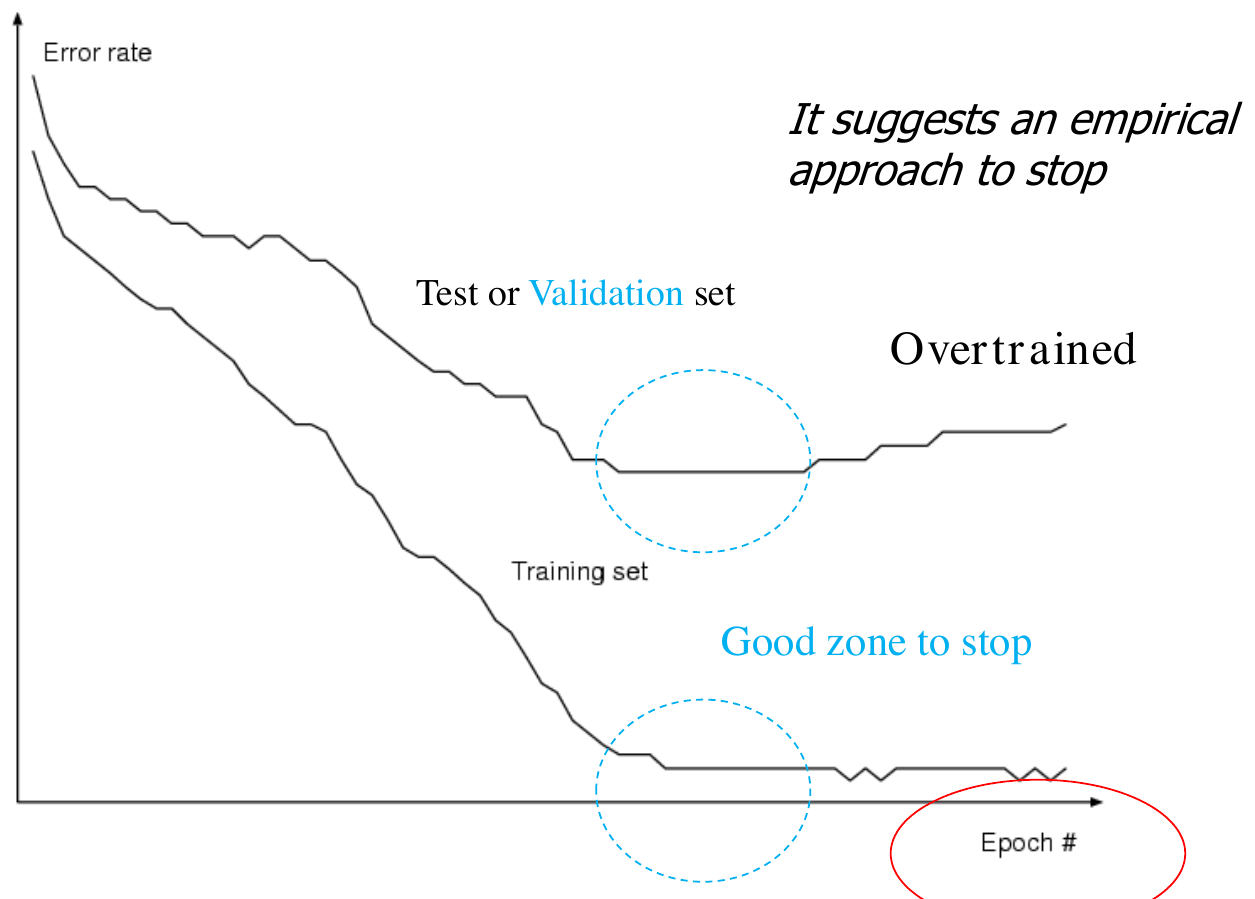
\includegraphics[width=0.63\linewidth,height=0.42\textheight,keepaspectratio]{images/08-nn2_early-stopping.png}
\caption{Comportamento tipico della backpropagation: suggerisce un criterio
empirico per fermarsi.}
\end{figure}

La curva va letta insieme al grafico del VC-bound (fondamento teorico).
Come intervenire:

\begin{enumerate}
\def\labelenumi{\arabic{enumi}.}
\tightlist
\item
  \textbf{Early stopping}: usare un \textbf{validation set} per decidere
  quando fermarsi, cioè quando l'errore di validazione inizia a salire.
  È vago: bisogna osservare più epoche prima di decidere
  (\emph{patience}) ed eventualmente tornare indietro
  (\emph{backtracking}). Poiché il numero effettivo di parametri cresce
  durante l'addestramento, \textbf{fermarsi prima equivale a limitare la
  complessità effettiva}.
\item
  \textbf{Regolarizzazione} della loss: il nostro strumento principale.
\item
  Metodi di \textbf{pruning} (più avanti).
\end{enumerate}

\subsection{Regolarizzazione (!)}\label{regolarizzazione}

Durante l'addestramento i pesi crescono: possiamo ottimizzare la loss
tenendo conto del loro valore. L'approccio fondato (di nuovo Tikhonov)
aggiunge un termine di penalità: \[
\text{Loss}(\mathbf{w}) = \sum_p\big(d_p - o(\mathbf{x}_p)\big)^2 + \lambda\,\|\mathbf{w}\|^2, \qquad \|\mathbf{w}\|^2 = \sum_i w_i^2 \text{ su tutti i pesi della rete.}
\] L'effetto è il \textbf{weight decay}: si aggiunge circa
\(2\lambda w\) al gradiente di ogni peso, \[
\mathbf{w}_{new} = \mathbf{w} + \eta\,\Delta\mathbf{w} - 2\lambda\mathbf{w}
\] (il 2 si può omettere). \(\lambda\) è in genere molto piccolo (es.
\(0{,}01\)) e si sceglie in \textbf{model selection} (cross-validation).
Applicata a un modello lineare è la ridge regression; esistono penalità
più sofisticate (ad esempio per la \emph{weight elimination}).

\begin{boxnote}{Errore e Loss}

Con un termine di penalità conviene distinguere: \textbf{Loss} è la
funzione obiettivo usata per l'addestramento (MSE + penalità);
\textbf{Errore/Rischio} è il termine sui dati (MSE), che misura l'errore
del modello. \textbf{(!)} È l'errore che va riportato in tabelle e
grafici, perché è la misura utile per chi usa il modello.

\end{boxnote}

\begin{figure}[htbp]
\centering
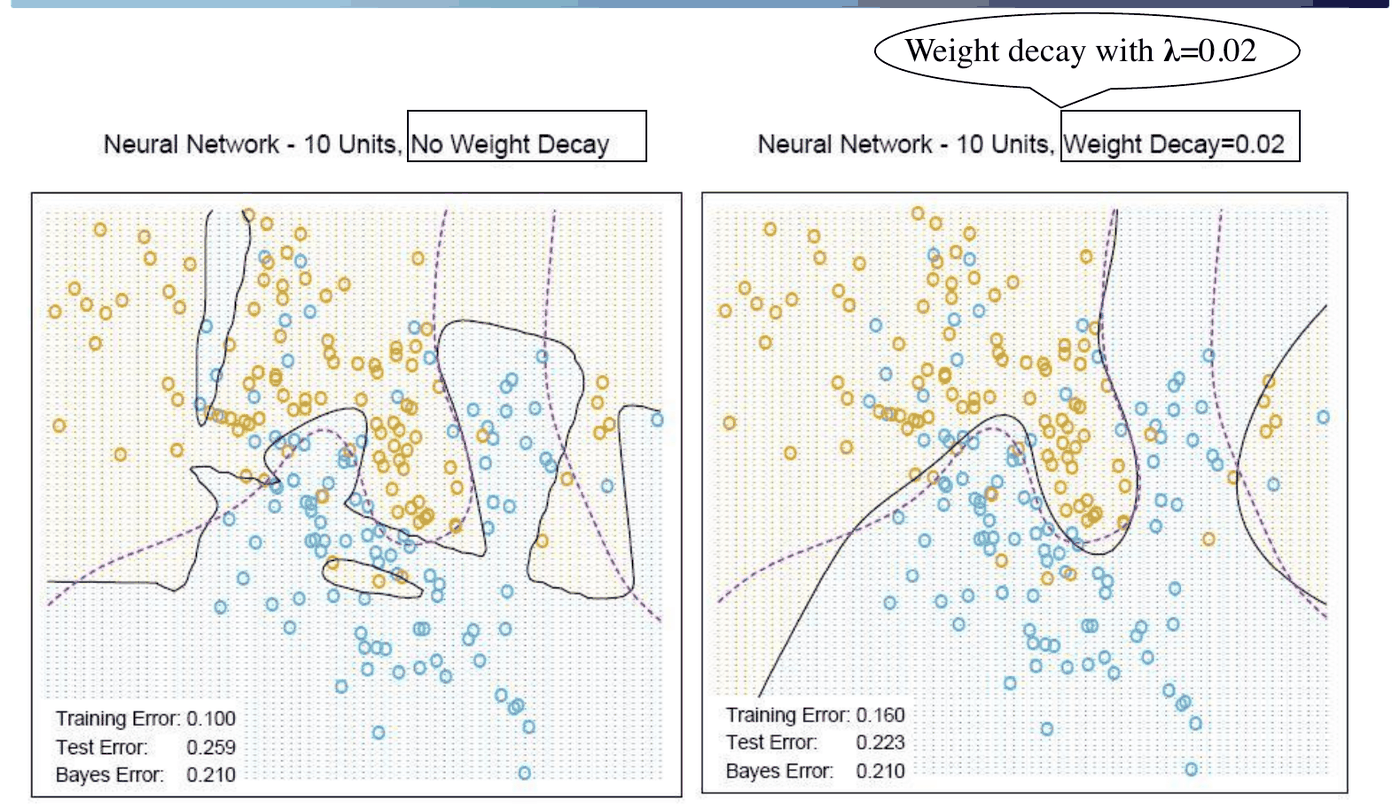
\includegraphics[width=0.91\linewidth,height=0.42\textheight,keepaspectratio]{images/08-nn2_weight-decay.png}
\caption{Effetto del weight decay su una rete da 10 unità
(Hastie-Tibshirani-Friedman): il confine diventa più regolare e l'errore
di test si avvicina a quello di Bayes (0,210).}
\end{figure}

\begin{figure}[htbp]
\centering
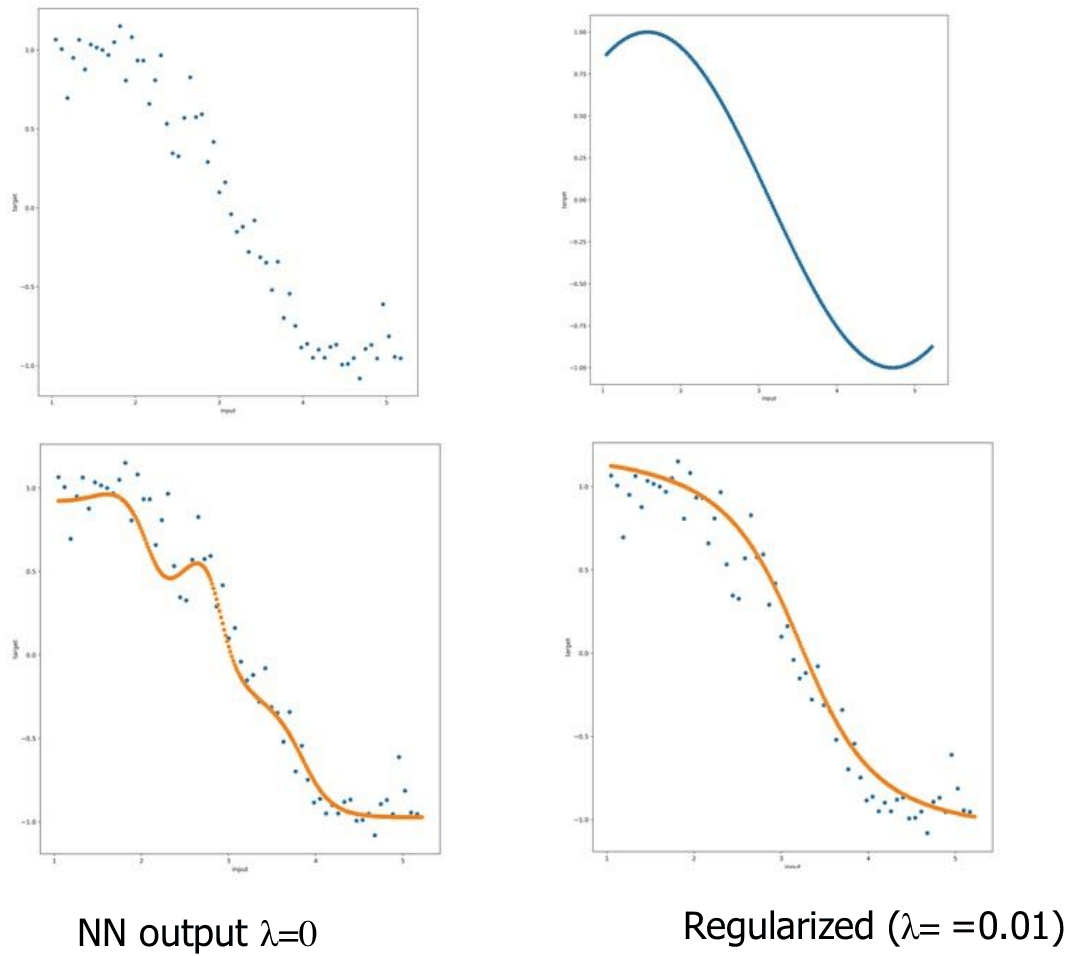
\includegraphics[width=0.63\linewidth,height=0.42\textheight,keepaspectratio]{images/08-nn2_regressione-reg.png}
\caption{Regressione univariata: rete senza regolarizzazione (\(\lambda = 0\)) e
regolarizzata (\(\lambda = 0{,}01\)).}
\end{figure}

\begin{figure}[htbp]
\centering
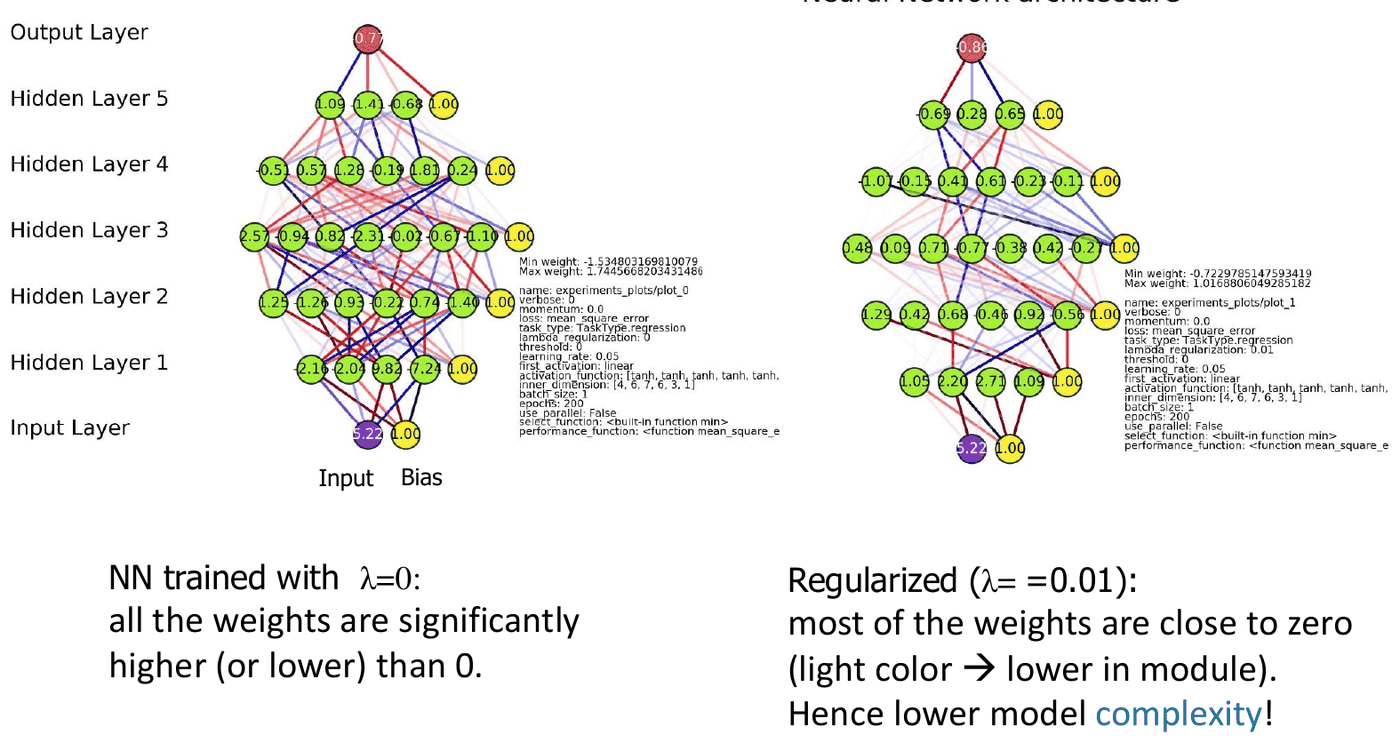
\includegraphics[width=0.91\linewidth,height=0.42\textheight,keepaspectratio]{images/08-nn2_pesi-reg.png}
\caption{I pesi della rete senza regolarizzazione (sinistra) e con
regolarizzazione (destra): con \(\lambda = 0{,}01\) la maggior parte dei
pesi è vicina a zero, quindi la complessità del modello è minore.}
\end{figure}

\subsubsection{Fraintendimenti
frequenti}\label{fraintendimenti-frequenti}

\begin{boxwarning}{La regolarizzazione non serve a stabilizzare la convergenza}

La regolarizzazione \textbf{non} è una tecnica per rendere più stabile
la curva di apprendimento: serve a \textbf{controllare la complessità}
del modello (misurata dalla VC-dim, legata al numero e al valore dei
pesi). Se la curva è instabile, il problema è altrove (learning rate,
batch\ldots).

\end{boxwarning}

\begin{boxquestion}{Meglio early stopping o regolarizzazione?}

L'early stopping è un approccio \textbf{empirico} che richiede un
validation set per decidere quando fermarsi, sacrificando una parte dei
dati. La regolarizzazione nella loss è un approccio \textbf{fondato}:
permette alla curva di validazione di seguire quella di training (purché
non si abbia underfitting per un \(\lambda\) troppo alto), e in quel
caso non serve (strettamente) l'early stopping e ci si può fermare a
convergenza. Si possono anche usare entrambi: l'early stopping non
interviene se l'errore di validazione non sale.

\end{boxquestion}

\subsubsection{Dettagli}\label{dettagli}

\begin{itemize}
\tightlist
\item
  Spesso il \textbf{bias \(w_0\) è escluso} dal regolarizzatore
  (includerlo renderebbe i risultati dipendenti da traslazioni/scalature
  del target), oppure ha un proprio coefficiente.
\item
  Tipicamente si applica nella versione batch. Nell'on-line/mini-batch
  la penalità viene applicata a ogni passo, quindi molte volte per
  epoca: per un confronto equo col batch si userebbe
  \(\lambda\cdot mb/l\). (Se \(\lambda\) si sceglie con la model
  selection, questo avviene automaticamente.)
\item
  Un'altra tecnica è il \textbf{dropout} (più avanti).
\end{itemize}

\subsection{Mettere tutto insieme: momentum e weight
decay}\label{mettere-tutto-insieme-momentum-e-weight-decay}

Con la loss regolarizzata, la regola con momentum diventa (separando i
due termini della loss e usando \(\eta\) solo per il termine d'errore,
come già fatto nei modelli lineari): \[
\Delta w_{tu} = -\eta\,\frac{\partial\,\text{Loss}}{\partial w_{tu}} + \alpha\,\Delta w_{tu}^{old} \;\doteq\; \eta\,\delta_t\,o_u - \lambda\,w_{tu} + \alpha\,\Delta w_{tu}^{old}, \qquad w_{tu}^{new} = w_{tu} + \Delta w_{tu}.
\] Così \(\eta\) non moltiplica \(\lambda\): cambiando uno non si cambia
l'altro.

Il momentum deve includere anche la parte di \(\lambda\)? Spesso sì
(Matlab, Caffe\ldots). Ma per rendere \textbf{indipendenti tutti e tre
gli iperparametri} \(\eta\), \(\alpha\), \(\lambda\) si può scrivere: \[
\Delta w_{tu} = \eta\,\delta_t\,o_u + \alpha\,\Delta w_{tu}^{old}, \qquad w_{tu}^{new} = w_{tu} + \Delta w_{tu} - \lambda\,w_{tu},
\] separando il weight decay dalla memoria del momentum. Si divide per
\(l\) solo il gradiente di \(E\) (dove c'è la somma sui pattern).

\section{Numero di unità nascoste}\label{numero-di-unituxe0-nascoste}

Il numero di unità è legato al \textbf{controllo della complessità},
alla dimensione dell'input e alla dimensione del training set. In
generale è un problema di \textbf{model selection}: il numero di unità,
insieme a \(\lambda\), si sceglie con la cross-validation.

\begin{itemize}
\tightlist
\item
  Troppe poche unità → underfitting; troppe → overfitting (può
  verificarsi).
\item
  Il numero di unità può essere più alto se si usa un'adeguata
  regolarizzazione.
\end{itemize}

Alternative alla ricerca manuale:

\begin{itemize}
\tightlist
\item
  \textbf{approcci costruttivi}: l'algoritmo decide il numero di unità
  partendo da una rete piccola e aggiungendone;
\item
  \textbf{metodi di pruning}: si parte da reti grandi e si eliminano
  progressivamente pesi o unità.
\end{itemize}

\subsection{Cascade Correlation}\label{cascade-correlation}

Tra gli approcci costruttivi (Tower, Tiling, Upstart per la
classificazione) il più noto è il \textbf{Cascade Correlation} (CC) di
Fahlman e Lebiere (1990), per regressione e classificazione. Apprende
\textbf{sia i pesi sia la topologia} (numero di unità): lo spazio delle
ipotesi ha dimensione flessibile, decisa dall'algoritmo, e a ogni passo
si addestra una sola unità.

\begin{boxabstract}{Algoritmo Cascade Correlation}

\begin{enumerate}
\def\labelenumi{\arabic{enumi}.}
\tightlist
\item
  Si parte da una rete \(N_0\) \textbf{senza unità nascoste} e la si
  addestra. Se non risolve il problema, si passa a \(N_1\).
\item
  In \(N_1\) si aggiunge un'unità nascosta i cui pesi vengono addestrati
  per \textbf{massimizzare la correlazione} tra la sua uscita e
  l'\textbf{errore residuo} della rete \(N_0\).
\item
  Dopo l'addestramento, i pesi in ingresso della nuova unità vengono
  \textbf{congelati}; si riaddestrano i pesi rimanenti (strato di
  uscita).
\item
  Se la rete non risolve il problema si aggiungono altre unità, ciascuna
  collegata a \textbf{tutti gli input e a tutte le unità nascoste
  precedenti} (da qui ``a cascata'').
\item
  Si continua finché l'errore residuo soddisfa il criterio di arresto.
\end{enumerate}

\end{boxabstract}

\begin{figure}[htbp]
\centering
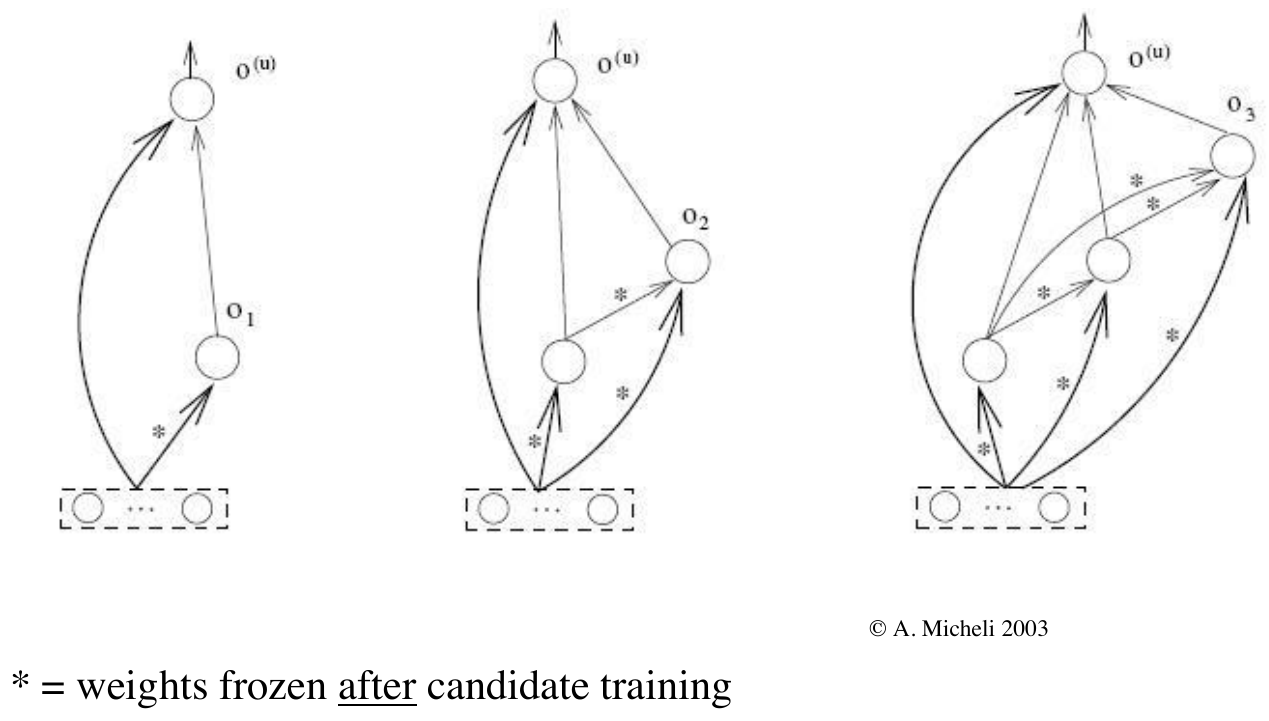
\includegraphics[width=0.74\linewidth,height=0.42\textheight,keepaspectratio]{images/08-nn2_cascade.png}
\caption{Costruzione di una rete Cascade Correlation con fino a 3 unità nascoste.}
\end{figure}

L'algoritmo alterna la minimizzazione dell'errore totale (LMS, ad
esempio backprop sullo strato di uscita) e la \textbf{massimizzazione
della covarianza} \(S\) tra l'uscita \(o_p\) della candidata e l'errore
residuo \(E_{p,k} = o_{p,k} - d_{p,k}\): \[
S = \sum_k\left|\sum_p\big(o_p - \bar{o}\big)\big(E_{p,k} - \bar{E}_k\big)\right|.
\] Il gradiente (con \(d|f|/dx = \operatorname{sign}(f)\,df/dx\) e
trascurando la dipendenza delle medie da \(o_p\)) è \[
\frac{\partial S}{\partial w_j} = \sum_k \operatorname{sgn}(S_k)\sum_p\big(E_{p,k} - \bar{E}_k\big)\,f'(net_{p,h})\,I_{p,j},
\] dove \(h\) è la candidata e \(I_{p,j}\) il suo input \(j\). Si fa
\textbf{ascesa} del gradiente (si massimizza \(S\)).

Note sul CC:

\begin{itemize}
\tightlist
\item
  il ruolo delle unità nascoste è \textbf{ridurre l'errore residuo}:
  ogni unità risolve un sotto-problema e diventa un \textbf{rilevatore
  di feature permanente};
\item
  \textbf{pool di candidate}: la superficie di \(S\) ha molti massimi,
  quindi si addestra un gruppo di candidate e si sceglie la migliore,
  evitando massimi locali;
\item
  è un algoritmo \textbf{greedy}: converge facilmente e può trovare un
  numero minimo di unità, ma può andare in overfitting (serve
  regolarizzazione);
\item
  la loss non deve essere necessariamente ``max \(S\)'' (per la
  regressione si può usare LMS).
\end{itemize}

\section{Input e output}\label{input-e-output}

\textbf{Input}: il pre-processing ha grande effetto.

\begin{itemize}
\tightlist
\item
  \textbf{Standardizzazione} (spesso utile): per ogni feature media 0 e
  deviazione standard 1, \((v - \text{media})/\text{dev. std}\).
\item
  \textbf{Rescaling} in \([0,1]\): \((v - \min)/(\max - \min)\).
\item
  Input categorici: codifica \textbf{1-of-K} (\(A \to 100\),
  \(B \to 010\), \(C \to 001\)).
\item
  Dati mancanti: attenzione, \textbf{0 non significa ``nessun input''}
  se 0 è nel range dei valori.
\end{itemize}

\textbf{Output}:

\begin{itemize}
\tightlist
\item
  \textbf{(!) Regressione}: unità di uscita \textbf{lineari} (una o
  più).
\item
  \textbf{Classificazione}: una unità (binaria) o 1-of-K con più uscite.
  Con la sigmoide si sceglie la soglia per assegnare la classe (con
  eventuale zona di rifiuto); con 1-of-K vince l'uscita più alta. Spesso
  la \textbf{tanh} (simmetrica) apprende più in fretta. Come target si
  può usare \(0{,}9\) invece di 1 (e \(-0{,}9\) o \(0{,}1\) invece di
  \(-1\) o \(0\)) per evitare la convergenza asintotica verso la
  saturazione. Ovviamente il range dei target deve stare nel range delle
  uscite.
\item
  \textbf{Softmax} per targets 0/1 multi-classe: le uscite sommano a 1 e
  si possono interpretare come probabilità
  \(p(\text{classe} = k \mid \mathbf{x})\): \[
  o_k(\mathbf{x}) = \frac{e^{net_k}}{\sum_{j=1}^{K} e^{net_j}}.
  \]
\item
  Si può usare la \textbf{cross-entropy} come loss alternativa (stima di
  massima verosimiglianza); per un'unità: \[
  -\sum_{i \in TR}\big\{d_i\log(out(\mathbf{x}_i)) + (1 - d_i)\log(1 - out(\mathbf{x}_i))\big\}.
  \]
\end{itemize}

\begin{boxquestion}{Esercizio per il progetto}

Riflettere sul ruolo dei diversi iperparametri e collegarli alla teoria:
ad esempio collegare la loss con penalità al VC-bound, per capire come
numero di unità, \(\lambda\) e gli altri controllano underfitting e
overfitting. Quali sono i più rilevanti per il progetto (e per vincere
la competizione)?

\end{boxquestion}

\section{Pregi e difetti delle reti
neurali}\label{pregi-e-difetti-delle-reti-neurali}

\begin{boxabstract}{Pregi}

\begin{itemize}
\tightlist
\item
  Metodo flessibile: estende i metodi lineari alla stima di funzioni
  arbitrarie e costruisce un'\textbf{ipotesi esplicita} (a differenza
  del K-NN).
\item
  Potere espressivo dato da numero di unità, architettura e
  addestramento.
\item
  Spazio delle ipotesi continuo e ricco, loss differenziabile →
  addestramento con discesa del gradiente.
\item
  Approssimatori universali; gestiscono rumore e dati incompleti con
  degrado graduale; dati continui e discreti, regressione e
  classificazione.
\item
  Un \textbf{paradigma} ampio (anche apprendimento non supervisionato,
  memorie associative, approcci stocastici).
\item
  Plausibilità neurale; \textbf{rappresentazione distribuita} della
  conoscenza (compatta in matrici di pesi); \textbf{tolleranza ai
  guasti}; adattamento a ambienti non stazionari con apprendimento
  on-line (\emph{continual learning}, con il dilemma
  stabilità-plasticità).
\end{itemize}

\end{boxabstract}

\begin{boxwarning}{Punti critici}

\begin{itemize}
\tightlist
\item
  \textbf{Problema della black box}: è difficile interpretare la
  conoscenza acquisita ed estrarla per gli esperti umani. È legato al
  tema attuale della \textbf{explainable AI} (XAI). Approcci:
  proiezione/clustering delle rappresentazioni interne, analisi di
  sensitività, \textbf{Layer-wise Relevance Propagation} (LRP, 2015,
  anche per reti profonde, che produce mappe di calore sulle parti
  dell'input rilevanti per la decisione), estrazione di regole
  simboliche.
\item
  \textbf{Progettazione dell'architettura}: servono metodi
  costruttivi/pruning o approcci diversi (SVM).
\item
  \textbf{Dipendenza dal processo di addestramento}: le molte varianti e
  iperparametri influenzano la soluzione finale.
\item
  Non ideali con \textbf{dati mancanti} (si usano rimozione,
  imputazione\ldots).
\end{itemize}

\end{boxwarning}

Le reti neurali sono indicate quando: l'input è ad alta dimensione
(discreto o reale), il task è di classificazione o regressione, i dati
possono essere rumorosi, il tempo di addestramento non è critico, la
forma della funzione target è sconosciuta, la leggibilità del risultato
non è critica, e il calcolo dell'uscita deve essere veloce.

\begin{boxnote}{Note storiche}

McCulloch e Pitts (1943), Hebb (1949), Minsky (1954, 1969), von Neumann
(1956), Rosenblatt (1958), Widrow e Hoff (1960), Kohonen (1972, 1982),
Grossberg (ART, 1980), Hopfield (1982), Rumelhart, Hinton, Williams,
Werbos, Parker, LeCun (1975--1985, backprop), Poggio e Girosi (teoria
RBF, 1990), Vapnik (SVM, anni '90), deep learning (Hinton, Bengio,
LeCun, dal 2007). \textbf{Hopfield e Hinton} hanno ricevuto il
\textbf{Premio Nobel per la Fisica 2024}; Hinton, Bengio e LeCun il
Premio Turing 2018.

\end{boxnote}

\section{Verso il progetto: il benchmark
MONK}\label{verso-il-progetto-il-benchmark-monk}

Non si è ancora pronti per il progetto (mancano la \textbf{validazione}
e la lezione dedicata), ma si può iniziare a implementare la rete
(backprop e regole di aggiornamento) o a esplorare i simulatori.

Verificare la correttezza di un'implementazione è difficile: una rete
spesso ``funziona'' (anche se male) nonostante piccoli errori. Il primo
collaudo è il dataset \textbf{MONK} (UCI), i cui risultati vanno
riportati nel report:

\begin{itemize}
\tightlist
\item
  3 task di classificazione binaria, piccoli e artificiali, ``non
  difficili'': una piccola rete con poche unità raggiunge accuratezze
  altissime (fino al 100\%) in poco tempo;
\item
  esiste un report con risultati precedenti di MLP e altri modelli;
\item
  \textbf{input}: 6 variabili con 2, 3 o 4 valori simbolici ciascuna →
  codifica \textbf{1-of-k} → \textbf{17 unità di input};
\item
  il test set include il training set (cattiva pratica, ma qui
  irrilevante).
\end{itemize}

\begin{boxtip}{Consigli per le prime prove sul MONK}

\begin{itemize}
\tightlist
\item
  Un'unità di uscita per la classificazione (target e uscite coerenti,
  \(0/1\) o \(-1/+1\)); si suggerisce la \textbf{tanh} in uscita.
\item
  \textbf{Codifica one-hot degli input}: errore frequentissimo se
  dimenticata!
\item
  Batch con gradiente diviso per il numero di pattern: converge in
  qualche centinaio di epoche.
\item
  Poche unità nascoste (2--5), come nel manuale: il test funziona se si
  raggiungono i risultati dello stato dell'arte con poche unità.
\item
  Il MONK è sensibile all'inizializzazione (poche unità): provare
  intervalli iniziali piccoli (o basati sul fan-in).
\item
  Con approcci on-line usare lo \textbf{shuffling} (i pattern sono
  ordinati per classe).
\end{itemize}

\end{boxtip}

Buoni risultati sul MONK \textbf{non garantiscono} la correttezza del
simulatore; risultati cattivi indicano \textbf{sicuramente} che codice o
impostazioni vanno rivisti. Nei grafici conta la \textbf{forma} delle
curve (lisce, convergenti), non i valori.

\begin{figure}[htbp]
\centering
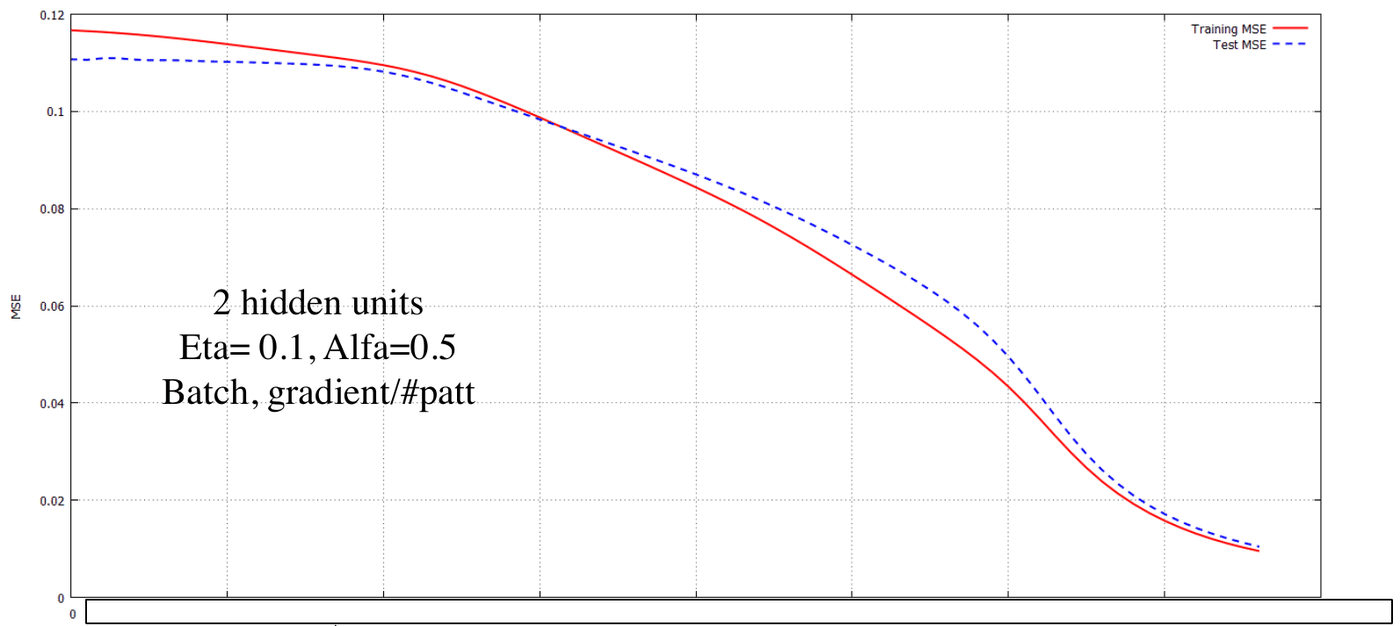
\includegraphics[width=0.80\linewidth,height=0.42\textheight,keepaspectratio]{images/08-nn2_monk2-mse.png}
\caption{MONK2: MSE di training (rosso) e test (blu tratteggiato) con 2 unità
nascoste, \(\eta = 0{,}1\), \(\alpha = 0{,}5\).}
\end{figure}

\begin{figure}[htbp]
\centering
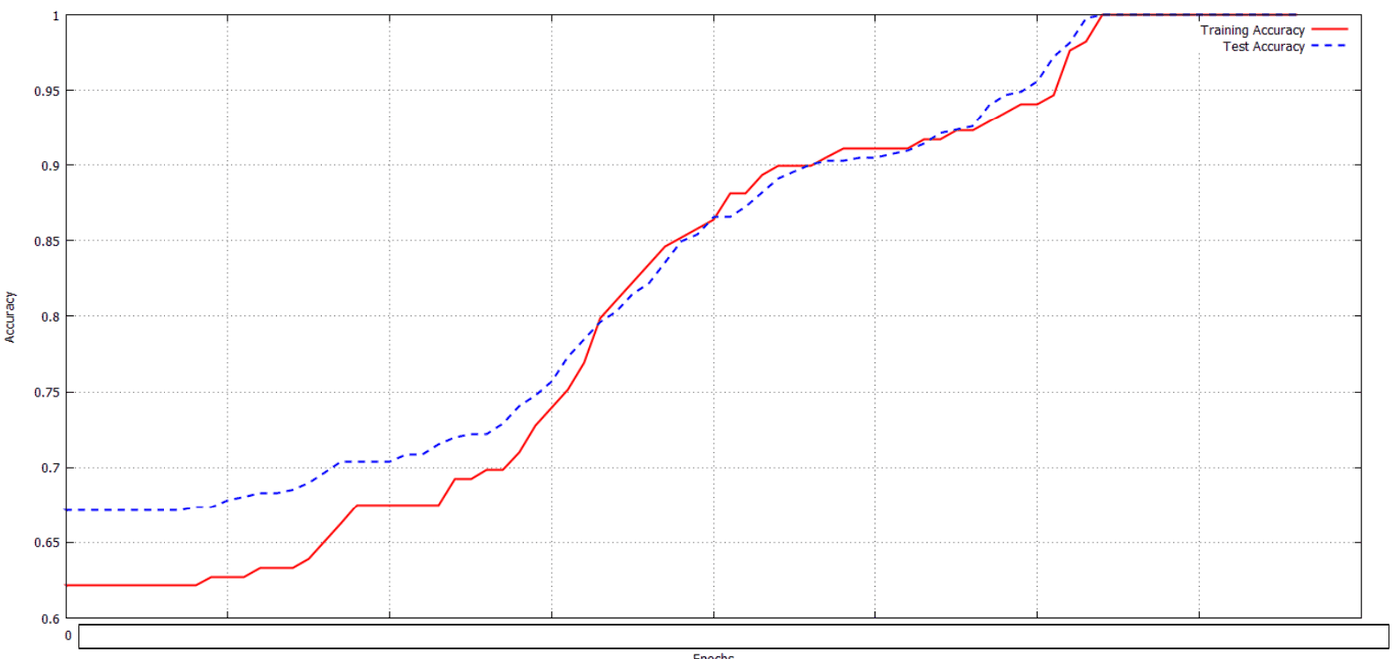
\includegraphics[width=0.80\linewidth,height=0.42\textheight,keepaspectratio]{images/08-nn2_monk2-acc.png}
\caption{MONK2: l'accuratezza raggiunge il 100\% anche sul test (caso insolito in
generale).}
\end{figure}

\begin{figure}[htbp]
\centering
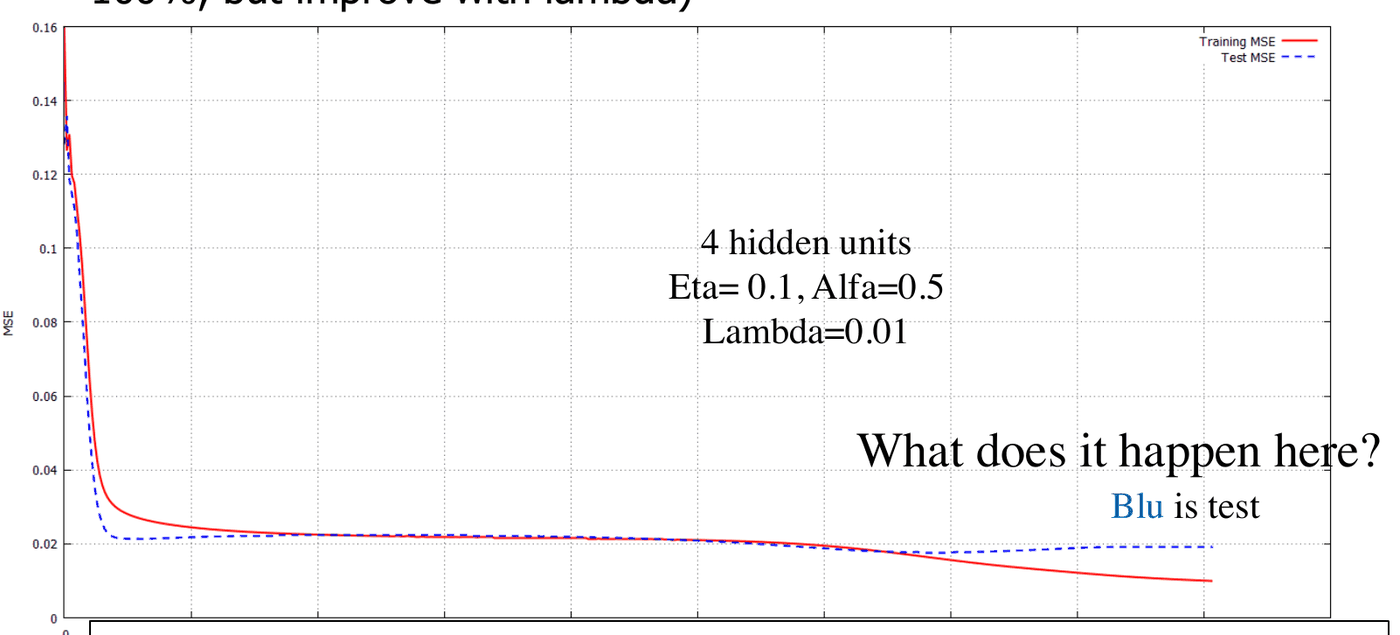
\includegraphics[width=0.80\linewidth,height=0.42\textheight,keepaspectratio]{images/08-nn2_monk3.png}
\caption{MONK3 con regolarizzazione (\(\lambda = 0{,}01\)): il MONK3 contiene
rumore e può andare in overfitting; il test non arriva al 100\%.}
\end{figure}

\begin{boxquestion}{Cosa succede nella Fig. 8.13?}

Nella parte finale l'errore di training continua a scendere mentre
quello di test risale leggermente: è l'inizio dell'\textbf{overfitting}
(MONK3 ha etichette rumorose). La regolarizzazione lo attenua; un
\(\lambda\) scelto con la model selection o l'early stopping
aiuterebbero.

\end{boxquestion}

Per verificare la backpropagation si può usare un esempio passo-passo
(attenzione se omette i bias) o una libreria affidabile come ``oracolo''
(Keras, scikit-learn, PyTorch\ldots). Altri dataset utili si trovano
nell'UCI Machine Learning Repository.

\begin{boxnote}{Anteprima del progetto (regole a.a. 2026/27)}

Negli anni passati il progetto era obbligatorio (gruppi di 2--3, tipo A
con simulatore implementato da zero o tipo B con librerie, competizione
ML-CUP). Dall'a.a. 2026/27 il progetto è \textbf{opzionale}: gruppi di
\textbf{2 studenti}, implementazione/applicazione/analisi di un metodo
di ML con valutazione sperimentale, presentato come \textbf{poster} in
una delle ultime lezioni (dicembre). Può dare un piccolo bonus ma non è
necessario per l'esame, che si basa sullo scritto (vedi
\href{01\%20-\%20Introduzione\%20al\%20Machine\%20Learning}{01 -
Introduzione al Machine Learning}). I consigli sul MONK restano validi
come collaudo di qualsiasi implementazione.

\end{boxnote}

\begin{boxquestion}{Possibili domande d'esame}

\begin{itemize}
\tightlist
\item
  Come si inizializzano i pesi e perché?
\item
  Differenze tra on-line, batch e mini-batch.
\item
  Ruolo del learning rate; cos'è il momentum e perché funziona?
\item
  Serve trovare il minimo globale? Perché?
\item
  Come si manifesta l'overfitting in una rete neurale? Cos'è l'early
  stopping?
\item
  Scrivere la loss con weight decay e la regola di aggiornamento con
  momentum.
\item
  La regolarizzazione migliora la stabilità della convergenza?
\item
  Descrivere il Cascade Correlation.
\item
  Come si rappresentano input e output per regressione e
  classificazione?
\end{itemize}

\end{boxquestion}
